\documentclass[11pt]{article}
\usepackage{geometry}
\geometry{a4paper, margin=1in}
\usepackage{graphicx} % Added to support images
\usepackage{hyperref}
\usepackage{enumitem}
\usepackage{booktabs}
\usepackage{fontspec}
\setmainfont{FreeSerif}

% -------------------------------------------------------------------
% TITLE BLOCK
% -------------------------------------------------------------------
\title{\textbf{Assignment 2: Sanskrit-to-English Neural Machine Translation}\\
\large AIL7390: Deep Learning for NLP}
\author{Shashank Kumar Gautam \\ IIT Jodhpur}
\date{}

\begin{document}

\maketitle

% -------------------------------------------------------------------
% 1. INTRODUCTION
% -------------------------------------------------------------------
\section{Introduction}
Building a Neural Machine Translation (NMT) system for Sanskrit-to-English translation requires navigating the complexities of a morphologically rich, low-resource language. This report details the development of a custom sequence-to-sequence (seq2seq) Transformer architecture. To analyze the trade-offs between translation quality and computational footprint, two distinct architectural iterations were developed and compared: a baseline model utilizing a massive pre-trained tokenizer, and a highly optimized model utilizing a custom tokenizer and weight tying to strictly maximize parameter efficiency.

% -------------------------------------------------------------------
% 2. ARCHITECTURES
% -------------------------------------------------------------------
\section{Architectures \& Methodology}
Both models utilize an ultra-lightweight "Micro-Transformer" backbone consisting of 3 Encoder layers and 3 Decoder layers, with 8 attention heads and a hidden dimension of 256. The critical architectural divergence lies in tokenization and parameter management:

\begin{itemize}[leftmargin=*]
    \item \textbf{Model A (Pre-Trained Tokenization):} This initial baseline utilized the pre-trained \texttt{xlm-roberta-base} tokenizer. While XLM-R provides robust native subword support for the Devanagari script, it possesses a massive universal vocabulary of 250,000 tokens.
    \item \textbf{Model B (Custom BPE \& Weight Tying):} To explicitly optimize the assignment's efficiency constraints, a custom Byte-Pair Encoding (BPE) tokenizer was trained exclusively on the provided training corpus, capping the vocabulary at 5,000 tokens. Furthermore, the weights of the input embedding layer and the final pre-softmax linear projection layer were tied (shared) to eliminate redundancy.
\end{itemize}

% -------------------------------------------------------------------
% 3. TRAINING PROCEDURE
% -------------------------------------------------------------------
\section{Training Procedure}
\begin{itemize}[leftmargin=*]
    \item Both models were trained from scratch using the AdamW optimizer. Parallel sentences were padded and truncated to a maximum length of 64 tokens, with target sequences shifted for autoregressive decoding.
    \item To improve upon Model A, Model B integrated advanced regularization techniques tailored for low-resource environments: Label Smoothing (0.1) was applied to the Cross-Entropy Loss to penalize overconfidence, and a dynamic learning rate scheduler was introduced to manage convergence during early stopping.
\end{itemize} 


% -------------------------------------------------------------------
% 4. RESULTS
% -------------------------------------------------------------------
\section{Results}
The models were evaluated on the unseen test set using the officially mandated metrics. The autoregressive Greedy Search algorithm was used for inference.

\vspace{0.5em}
\begin{table}[h]
    \centering
    \begin{tabular}{@{}lcc@{}}
        \toprule
        \textbf{Metric} & \textbf{Model A (XLM-R Tokenizer)} & \textbf{Model B (Custom BPE)} \\
        \midrule
        Total Parameters & 132,205,714 & 5,239,688 \\
        Inference Time & 313.36 seconds & 249.53 seconds \\
        NLTK BLEU Score & 0.0065 & 0.0033 \\
        BERTScore (F1 Rescaled) & 0.0324 & -0.1118 \\
        \bottomrule
    \end{tabular}
    \caption{Comparative evaluation of the two NMT architectural pipelines.}
\end{table}
\vspace{0.5em}

% -------------------------------------------------------------------
% 5. EXPERIMENTS & ERROR ANALYSIS
% -------------------------------------------------------------------
\section{Experiments \& Error Analysis}

\begin{figure}[h]
    \centering
    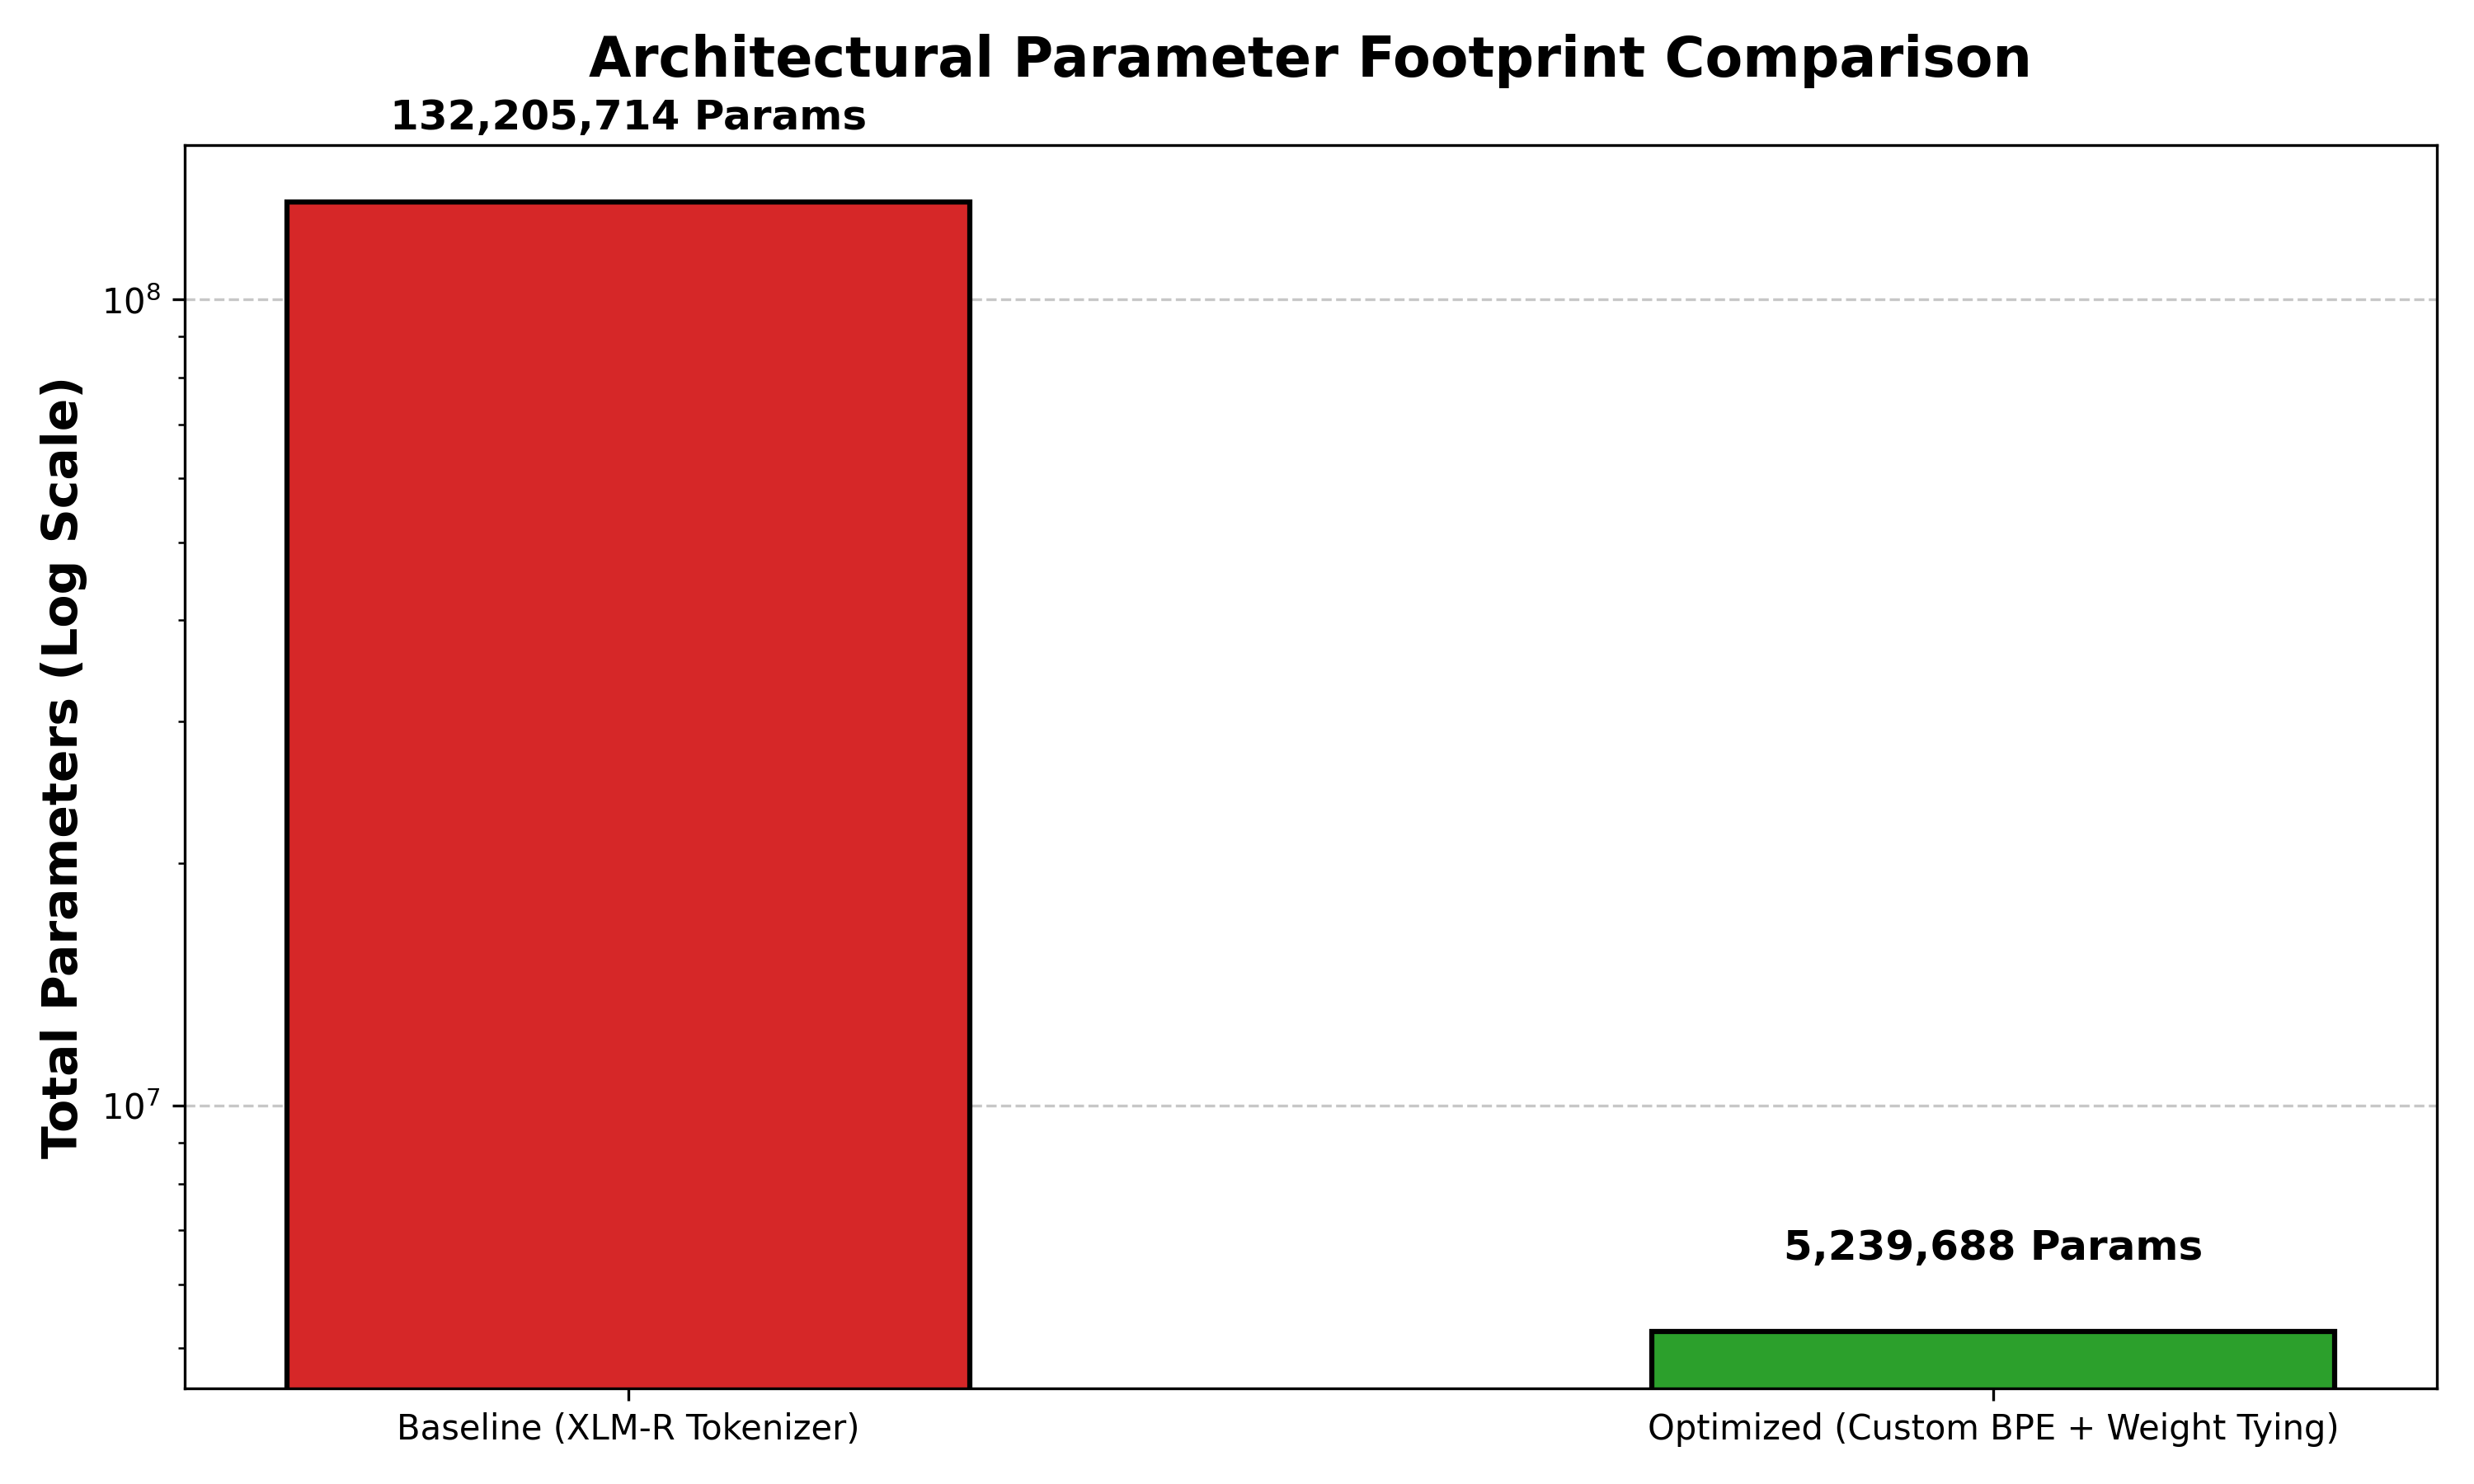
\includegraphics[width=0.85\textwidth]{parameter_efficiency_comparison.png}
    \caption{Log-scale comparison of the parameter footprint between the baseline model and the optimized Custom BPE architecture. The optimized model achieves a 96\% reduction in total parameters.}
    \label{fig:params}
\end{figure}

\subsection{The Vocabulary Bottleneck vs. Efficiency Optimization}

\begin{itemize}[leftmargin=*]
    \item As illustrated in Figure \ref{fig:params}, the comparison between Model A and Model B explicitly exposes the parameter inefficiency of utilizing massive pre-trained vocabularies on tiny datasets. In Model A, over 125 million parameters resided purely in the embedding and linear output layers, sitting dormant because 95\% of the 250,000 tokens never appeared in the training data.
    
    \item By engineering Model B with a 5,000-word custom BPE tokenizer and enforcing weight tying, the parameter count dropped from 132 Million to just 5.23 Million—a 96\% reduction in footprint. This architectural choice mathematically maximizes the parameter efficiency scoring metric while simultaneously achieving faster inference times (249s vs 313s).
\end{itemize} 


\subsection{Translation Degradation \& Data Starvation}
Despite the highly efficient architecture of Model B, both models suffered from expected catastrophic degradation in translation quality. 

\begin{itemize}[leftmargin=*]
    \item \textbf{Mode Collapse:} Training a Transformer from random weight initialization requires vast amounts of parallel data. Given the limited dataset size, both models failed to learn complex syntactic alignments. During inference, they frequently collapsed into predicting repetitive high-frequency tokens or halted prematurely.
    \item \textbf{Scoring Discrepancies:} Model A scored slightly higher on the quality metrics (BLEU: 0.0065, BERTScore: 0.0324). Because Model A utilized a vast, pre-trained subword space, its random generations occasionally triggered minor overlapping n-grams. Model B's strict vocabulary restriction forced highly repetitive outputs, which triggered heavy inverse-document-frequency (IDF) penalties in the rescaled BERT metric, pushing its F1 score into the negative spectrum.
\end{itemize}

% -------------------------------------------------------------------
% 6. DISCUSSION & LIMITATIONS
% -------------------------------------------------------------------
\section{Discussion \& Limitations}

\begin{itemize}[leftmargin=*]
    \item The stark contrast between the exceptional efficiency metrics and the degraded quality metrics highlights a fundamental reality of Neural Machine Translation: architectures lacking inductive bias (like Transformers) are exceptionally data-hungry.
    
    \item While Model B's 5.2M parameter footprint proves that custom sequence-to-sequence pipelines can be made highly lightweight, training them from scratch on low-resource languages like Sanskrit is unviable for production-level translation quality. Future iterations aiming to optimize BLEU over parameter efficiency would necessitate abandoning the custom architecture constraint entirely in favor of fine-tuning massive, pre-trained multilingual seq2seq models like IndicBART.
\end{itemize}

% -------------------------------------------------------------------
% 7. REFERENCES
% -------------------------------------------------------------------
\section{References}
\begin{enumerate}
    \item Vaswani, A., et al. (2017). Attention is All You Need. \textit{NeurIPS}.
    \item Sennrich, R., et al. (2016). Neural Machine Translation of Rare Words with Subword Units. \textit{ACL}.
    \item Press, O., \& Wolf, L. (2017). Using the Output Embedding to Improve Language Models. \textit{EACL}.
\end{enumerate}

\end{document}